\documentclass[../main.tex]{subfiles}

\begin{document}
    
    %%%%%%%%%%%%%%%%%%%%%%%%%%%%%%%%%%%%%%
    
    
    El fenómeno de fusión nuclear, consiste en acercar los núcleos de 2 átomos, para que puedan reaccionar y convertir masa en energía, a través de la ecuación de equivalencia entre masa y energía $E=mc^2$. Para esto, es conveniente que la carga de los núcleos (carga positiva) sea pequeña. Esto se traduce en un número atómico bajo, pues significa que tendremos una menor cantidad de protones que se repelen entre sí, y la repulsión eléctrica será menor. Para disminuir aún más la distancia a la que se aproximan unos de otros, es necesario que las partículas estén sometidas a altas temperaturas. Una vez que estén lo suficientemente cerca, la fuerza nuclear fuerte (fuerza de corto alcance) tendrá 
    mayor predominancia frente a la fuerza eléctrica. Entonces, ambos nucleos se fusionarán en uno solo, de menor masa, y se liberarán otras partículas adicionales, como neutrones energéticos. Es importante tener en cuenta, que no todos los núcleos son fusionables. Debido a la distinta naturaleza de las interacciones eléctrica y nuclear fuerte, a medida que aumentemos el número de nucleones, por ejemplo, agregando más protones al núcleo, la repulsión entre estos aumentará. Además, no todos estarán a la distancia requerida para que la fuerza nuclear fuerte pueda mantenerlos unidos. Por lo tanto, a partir de cierto número de nucleones, la adición de un protón o neutrón provocará que este sea inestable, y se dividirá o fisionará, liberando energía en el proceso. Estos fenómenos nucleares dependen del número de nucleones, como se puede ver en la Fig \ref{fig: fusion_fision}.
    
     \begin{figure}[h]
        \centering
        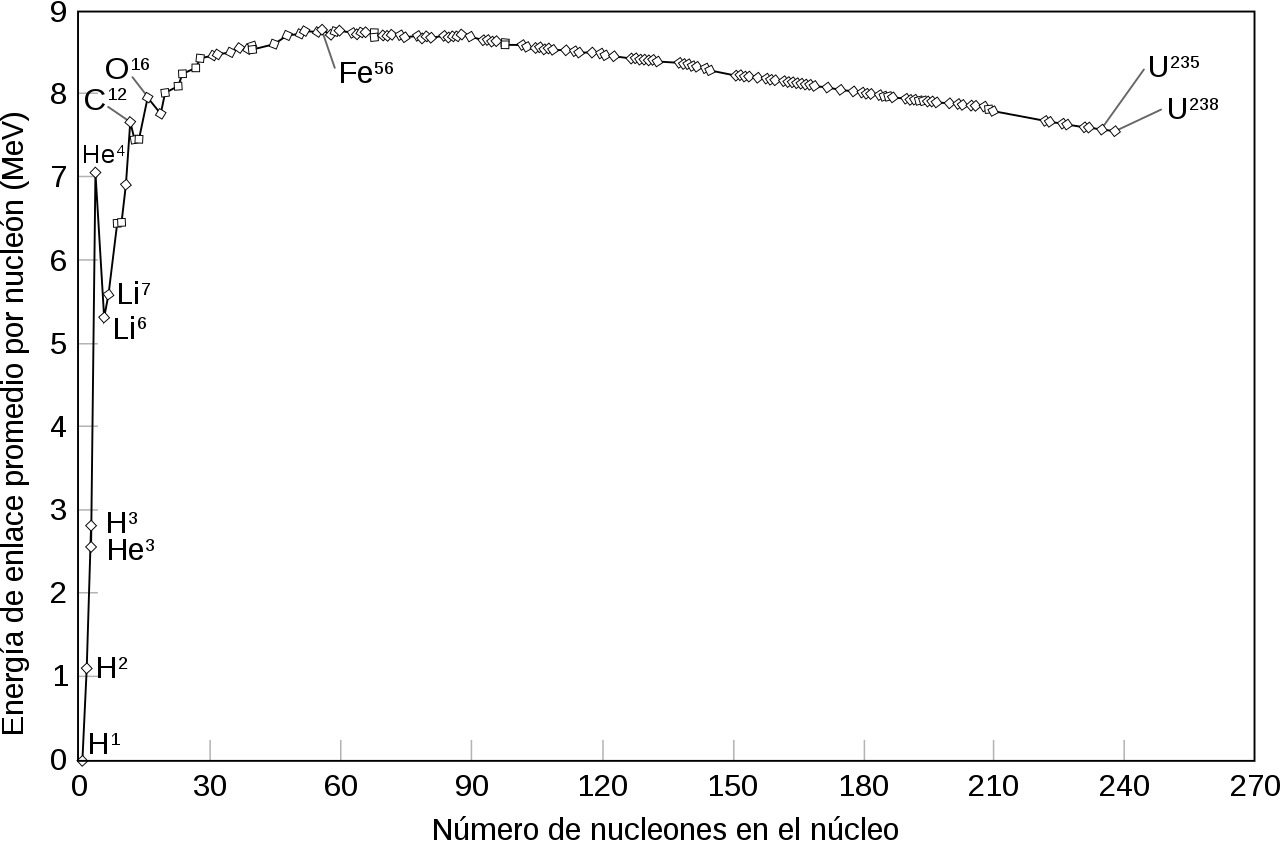
\includegraphics[width=0.9\textwidth]{Images/energia_de_enlace.jpg}
        \caption{A medida que aumente el número de nucleones en un núcleo, este se volverá más grande, y la distancia entre algunos protones superará la máxima distancia en donde la fuerza nuclear actúa. Debido a que la fuerza de repulsión eléctrica será mayor que la fuerza nuclear fuerte, el núcleo se volverá inestable. Tenemos entonces que, el núcleo de $\mathrm{Fe}^{56}$, es el elemento más estable de todos, pues se tendrá la máxima energía de enlace por núcleon, es decir, se tendrá una máxima unión, y por lo tanto, una máxima estabilidad.}
        \label{fig: fusion_fision}
    \end{figure}
	%%%%%%%%%%%%%%%%%%%%%%%%%
    \section{Reaccciones de Fusión }
	\lhead[\thepage]{\thesection. Reacciones de Fusión}

	Cada proceso de fusión es distinto, en cuanto a las partes que se fusionan y los productos. Para una reacción de fusión D-T o
    deuterio ($\mathrm{\tensor[^2]{H}{}}$) - tritio ($\mathrm{\tensor[^3]{H}{}}$), calculamos la energía liberada por reacción considerando el déficit de masa al final del proceso. Para esto, denotamos como $\mathrm{m_p}$ y $\mathrm{m_n}$, las masas del protón y neutrón respectivamente. Dado que el deuterio está formado por un protón y un neutrón, y el tritio, por un protón y dos neutrones, planteamos la ecuación de balance, y las masas respectivas para cada nucleón en función de $\mathrm{m_p}$
    \begin{align}
        \mathrm{m_p} &= 1.007276 \  \mathrm{uma}, \\
        \mathrm{m_n} &= 1.008665 \ \mathrm{uma} = 1.001378 \ \mathrm{m_p}, \\
        \mathrm{m_{\tensor[^2]{H}{}}} &= 2.014101 \ \mathrm{uma} = 1,999552 \ \mathrm{m_p}, \\
        \mathrm{m_{\tensor[^3]{H}{}}}  &= 3.016049 \ \mathrm{uma} = 2,994263 \ \mathrm{m_p}, \\
        \mathrm{m_{He}} &= 4.002602 \ \mathrm{uma} = 3,973689 \ \mathrm{m_p},
    \end{align}
    donde $\mathrm{m_p=1.007276 \ uma = 1,6726\times10^{-27} \ kg}$. Luego
    \begin{align}
        \mathrm{\tensor[^2]{H}{}+\tensor[^3]{H}{} &\longrightarrow  \mathrm{\tensor[^4]{He}{}+\tensor[^1]{n}{}}}, \\
        \mathrm{1,999552 \ m_p} + \mathrm{2,994263 \ m_p} &\longrightarrow \mathrm{3,973689 \ m_p} + \mathrm{1.001378 \ m_p}.
    \end{align}
    El déficit de masa $\Delta m$ será entonces
    \begin{align}
        &\Delta m = m_{total \ final}-m_{total \ inicial}, \\
        &\Delta m = \left(\mathrm{3,973689 \ m_p} + \mathrm{1.001378 \ m_p}\right) - \left(\mathrm{1,999552 \ m_p} + \mathrm{2,994263 \ m_p}\right), \\
        &\Delta m = \mathrm{4,975067 \ m_p - 4,993815\ m_p}, \\
        &\Delta m = -\mathrm{0,018748 \ m_p}.
    \end{align}
    El signo negativo es debido a que hubo una perdida de masa en el proceso. Esa masa será la energía liberada por la reacción. Entonces
    \begin{align}
        &E = \left|\Delta m\right|c^2, \\
        &E = \mathrm{0,018748\times 1.6726\times10^{-27} \ kg \times \left(299 \ 792\times10^3 \ ms^{-1}\right)^2}, \\
        &E = 2.818\times10^{-12} \ \mathrm{J} = 17.59 \ \mathrm{MeV},
    \end{align}
    donde $\mathrm{c} = 299 \ 792 \ \mathrm{km \ s^{-1}}$ y $1 \ \mathrm{J} \equiv 6.242\times10^{12} \ \mathrm{MeV}$. Entre otros procesos tenemos
        \begin{align}
        \mathrm{\tensor[^2]{H}{}+\tensor[^2]{H}{} &\longrightarrow  \mathrm{\tensor[^3]{H}{}+\tensor[^1]{H}{}}}, \\
        \mathrm{1,999552 \ m_p} + \mathrm{1.999552 \ m_p} &\longrightarrow \mathrm{2.994263 \ m_p} + \mathrm{1.000545 \ m_p}, \\
        E &= \mathrm{4.031 \ MeV},
        \end{align}
        \begin{align}
        \mathrm{\tensor[^2]{H}{}+\tensor[^2]{H}{} &\longrightarrow  \mathrm{\tensor[^3]{He}{}+\tensor[^1]{n}{}}}, \\
        \mathrm{1,999552 \ m_p} + \mathrm{1.999552 \ m_p} &\longrightarrow \mathrm{2.994243 \ m_p} + \mathrm{1.001378 \ m_p}, \\
        E &= \mathrm{3.268 \ MeV}
        \end{align}
        \begin{align}
        \mathrm{\tensor[^2]{H}{}+\tensor[^3]{He}{} &\longrightarrow  \mathrm{\tensor[^4]{He}{}+\tensor[^1]{H}{}}}, \\
        \mathrm{1,999552 \ m_p} + \mathrm{2.994263 \ m_p} &\longrightarrow \mathrm{3.973689 \ m_p} + \mathrm{1.000545 \ m_p}, \\
        E &= \mathrm{18.37 \ MeV}.
        \end{align}
  
	%-----------------------------------------

  % \section{Temperatura y densidades }
  % \lhead[\thepage]{\thesection. Temperatura %y densidades}
   
   %------------------------------------------

    \section{Sección Tranversal y velocidad de reacción}
	\lhead[\thepage]{\thesection. Sección Tranversal y velocidad de reacción}
	%------------------------------------------
	Para que se de lugar a una reacción de fusión, las partículas (núcleos) involucrados en las reacciones mencionadas anteriormente, deben vencer la repulsión electrostática debido a sus cargas positivas  
	
	\begin{align} \label{equ1}
	    V = \frac{e^2}{4\pi\epsilon_0}\frac{Z_XZ_Y}{r}.
	\end{align}
	
	La energía de interacción, o específicamente, la energía de repulsión, aumenta a medida que la distancia $r$ entre ambos núcleos disminuye, según (\ref{equ1}). A una cierta distancia, esta energía cae abruptamente hasta un valor negativo, debido a que se manifiestan interacciones ajenas a la electrostática (Interacción Fuerte). Tenemos entonces, que la interacción pasa a ser atractiva. Este límite se conoce como Barrera de Coulomb, y depende del número de protones en el núcleo, y el radio del mismo. La altura de la barrera se determina en la distancia entre ambos nucleos, igual a la separación de sus centros, y asumiendo que tienen simetria esférica y una densidad casi constante. Para núcleos con bajo número atómico se puede usar la aproximación (\ref{equ2}) para el radio nuclear \cite{krane1987introductory}, y reemplazando en (\ref{equ1}), tenemos que
	
	\begin{align} \label{equ2}
	    &R_A = r_0A^{1/3}, \\
	    &V_{XY} = \frac{e^2}{4\pi\epsilon_0}\frac{Z_XZ_Y}{(R_X + R_Y)},
	\end{align}
	
	donde
	\begin{itemize}
	    \item $R_A$: Radio atómico
	    \item $r_0$: Factor numérico igual \mathrm{$1.25 x 10^{-15} \ m$}
	    \item $A$: Número de nucleones (Protones y Neutrones)
	\end{itemize}
	
	\begin{figure}[h]
        \centering
        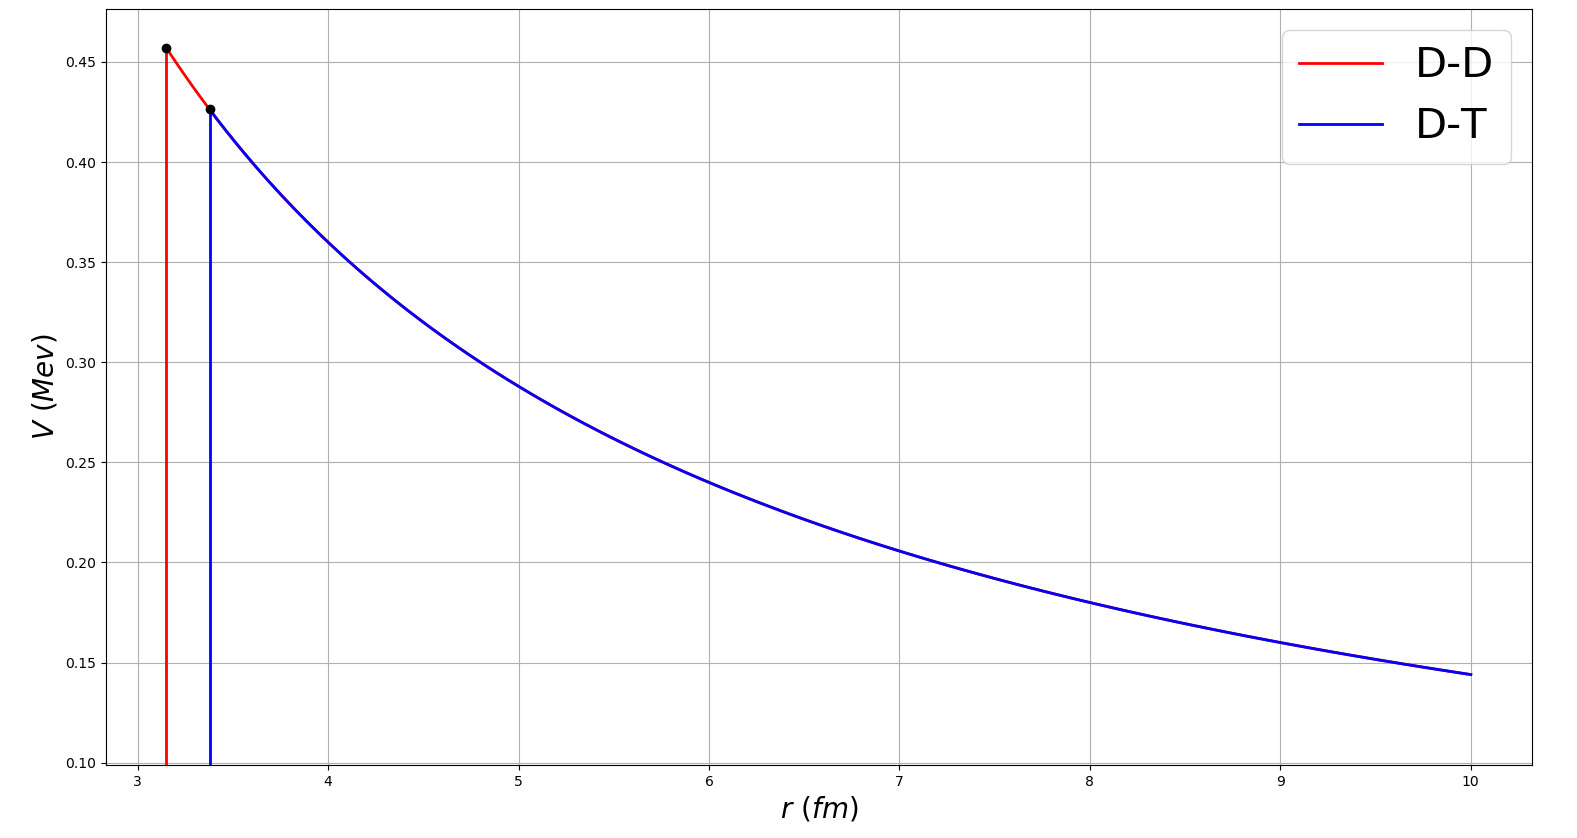
\includegraphics[width=16cm, height=9cm]{barrera_coulomb.jpg}
        \caption{Barrera de Coulomb para reacciones D-D y D-T. Se tomo $Z_D =Z_T = 1$, $A_D = 2$, $A_T=3$. Los ejes $x$ e $y$ están medidos en femtómetros ($fm$) y $MeV$. }
        \label{fig:imagen1}
    \end{figure}
	
	Para poder fusionar ambos núcleos en una reacción, es necesario que las partículas tengan suficiente energía cinética como para vencer la barrera de Coulomb mostrada en la figura (Figura \ref{fig:imagen1}). Sin embargo, existe otro factor importante para que se de una reacción de fusión. Ambos núcleos necesitan aproximarse entre sí dentro de cierto margen o sección transversal. Para entender esto imaginemos que dos partículas colisionan si, una de ellas cae dentro de cierta área representativa para la otra partícula. Si tomamos un haz de partículas que se dirige hacia otra partícula en reposo (Figura \ref{fig:sec_trans1}), con velocidad $v$, durante cierto intervalo de tiempo $dt$, el número de partículas en el haz que logran atravesar el área o sección transversal de la otra partícula, se calcula como
	
	\begin{align} \label{equ3}
	    N_p = n\sigma v dt,
	    \label{numero_part_cilindro}
	\end{align}
	
	donde $n$ es la densidad de partículas en el haz, y $\sigma$ es el área de la sección transversal de la partícula impactada. Para este modelo simplificado, observamos que el número de partículas que colisionan, es proporcional a la velocidad del haz y a la sección transversal de la partícula objetivo. Podemos decir entonces que, el número de reacciones depende de estas dos magnitudes. Para un gas de plasmas, sin embargo, esta dependencia es diferente a la del modelo mostrado, debido a que las condiciones son distintas (Figura \ref{fig:sec_trans2}). Primero, no se tiene una partícula como objetivo definido, ni un haz de partículas que impacte sobre esta. En su lugar, se tiene un gas de partículas cargadas con velocidades aleatorias, tanto en dirección como en magnitud. Aún así, la dependencia en la velocidad y sección transversal se mantiene.\\
	
	\begin{figure}[h] 
        \centering
        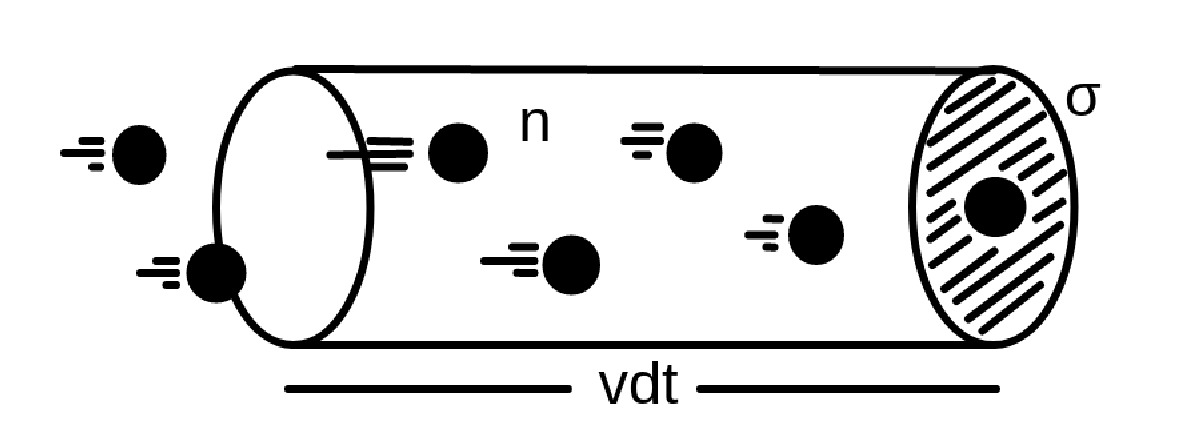
\includegraphics[width=0.7\textwidth]{Images/cap3_1.jpg}
        \caption{El número de partículas que colisionarán con la partícula en reposo, será igual al número de partículas que atraviesen su sección transversal $\sigma$. Se asume una densidad constante en el haz, y que todas las partículas tienen la misma velocidad $v$.}
        \label{fig:sec_trans1}
\end{figure}
\begin{figure}[h] 
        \centering
        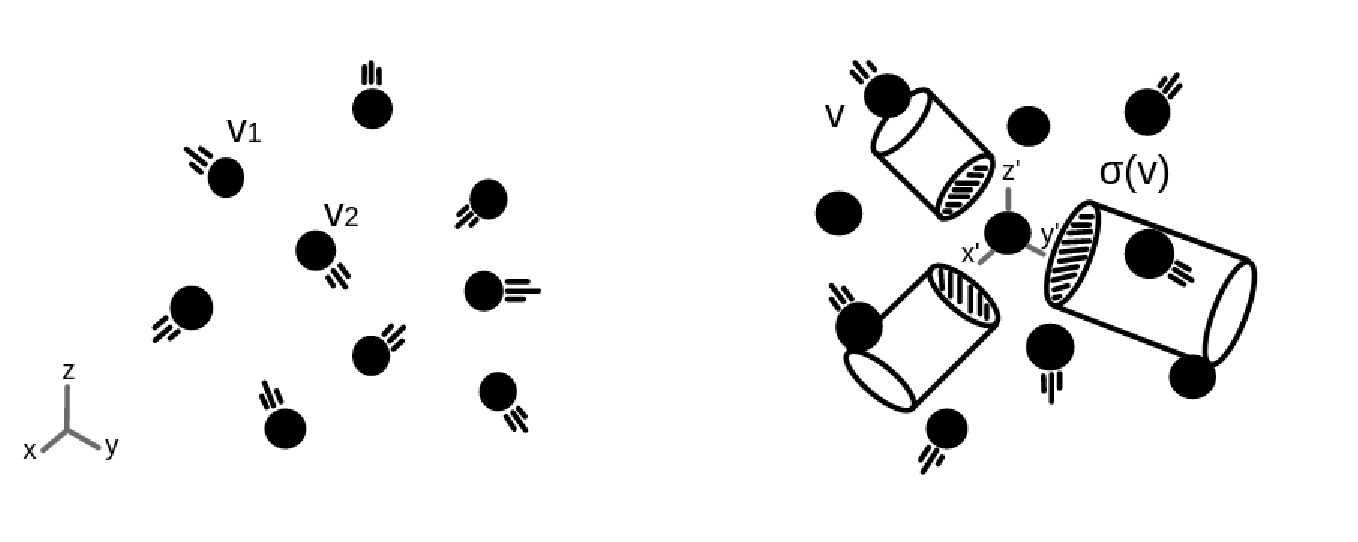
\includegraphics[width=0.8\textwidth]{Images/cap3_2.jpg}
        \caption{En un plasma, las partículas tienen velocidades aleatorias. Por lo tanto, se puede definir una sección transversal característica para cada dirección. El efecto total será la integración de todas ellas.}
        \label{fig:sec_trans2}
\end{figure}
	
	Para un núcleo dentro del plasma, se puede considerar el movimiento relativo de los demás núcleos respecto del primero, el cual se considera como el núcleo objetivo. Entonces, tendremos una velocidad relativa $v'$, cuya dependencia en el número de reacciones de fusión radica en que, la probabilidad de que se de el proceso depende de cuantos núcleos impacten al objetivo. De (\ref{numero_part_cilindro}), vemos que para el mismo intervalo de tiempo $dt$, el número de núcleos que impacten será mayor si $v'$, en nuestro caso, es mayor. Además, dado que no se tiene haces de partículas definidos, se puede construir una sección transversal en cada dirección de impacto por parte de las partículas circundantes.
	Esta dirección dependerá de la velocidad de las mismas, por lo que la sección transversal dependerá también de $v'$. \\
	
	Dicho esto, definimos la velocidad de reacción de fusión por unidad de volumen entre dos especies de partículas, con velocidades $v_1$ y $v_2$ como
	
	\begin{align}
	    R' = n_1n_2\sigma(v')v'f_1(\mathbf{v_1})f_2(\mathbf{v_2}),  
	\end{align}
	
	donde $f(\mathbf{v})$ y $v'$ son la distribución de Maxwell para las velocidades, y la velocidad relativa de la especie 1 respecto de la especie 2
	
	\begin{align}
	    &f\left(\mathbf{v}\right) = n\left(\frac{m}{2\pi k_BT}\right)^{3/2}exp\left(-\frac{mv^2}{2k_BT}\right), \\
	    &v'= \left|\mathbf{v_1} - \mathbf{v_2} \right|.
	\end{align}
	
	La velocidad de reacción total por unidad de volumen se obtiene integrando sobre todas las velocidades, por lo que se tiene que
	
	\begin{align}
	    &R = n_1n_2\iint\sigma(v')v'f_1(\mathbf{v_1})f_2(\mathbf{v_2})d^3v_1d^3v_2, \label{equ4} \\
	    &R = n_1n_2\left<\sigma v' \right> \label{equ5}
	\end{align}
	
	La ecuación (\ref{equ5}) tiene cierta similtud con (\ref{numero_part_cilindro}), dado que se observa la proporcionalidad respecto de $\sigma v$. En el caso de un plasma, con muchas partículas cargadas y velocidades aleatorias, esta proporcionalidad se refleja en un promedio sobre este producto. Así, la velocidad de reacción por unidad de volumen y por unidad de tiempo nos dice qué tan rápido ocurren estas reacciones, mientras que la sección transversal $\sigma$, es una medida de la probabilidad de que ocurra una reacción de fusión. 
	
	\begin{figure}[h]
        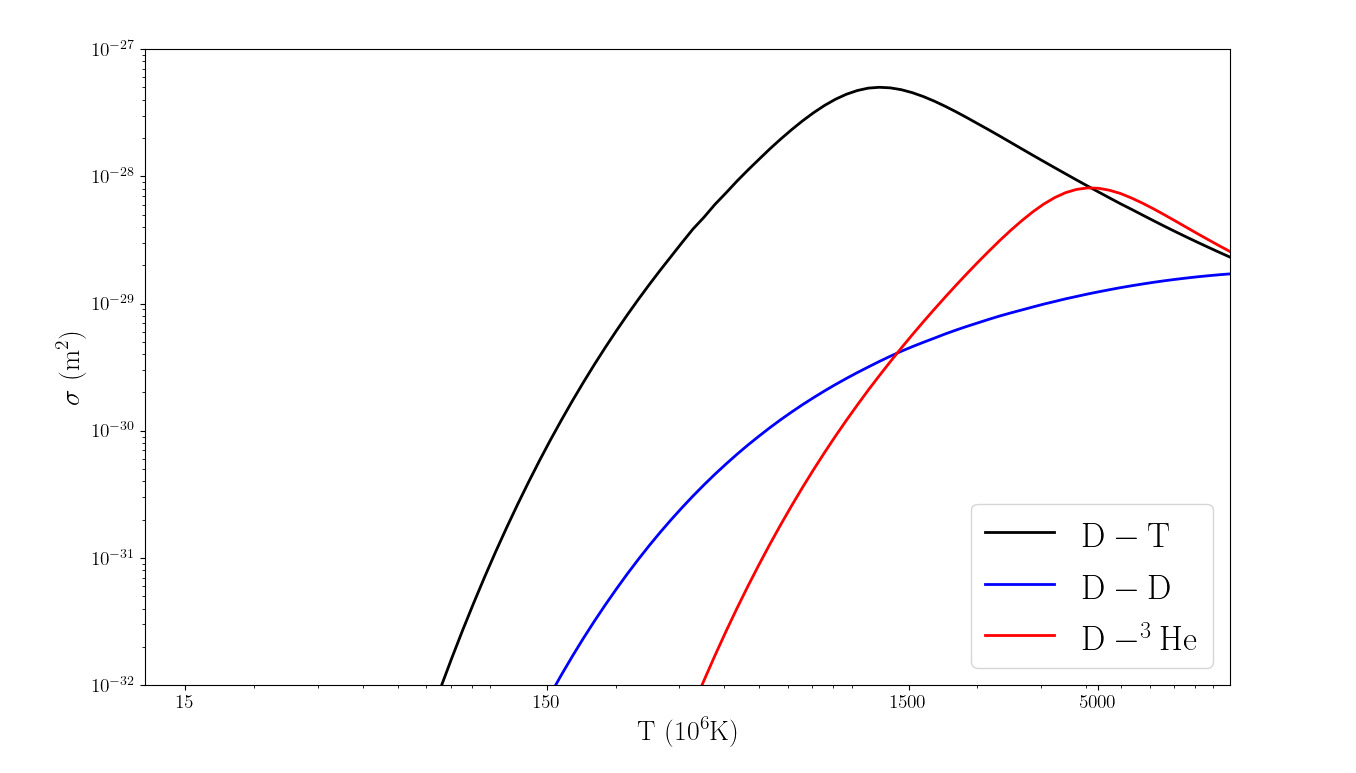
\includegraphics[width=16cm, height=9cm]{cross_section.jpg}
        \caption{Sección transversal para distintas reacciones de fusión.}
        \label{fig:mesh1}
    \end{figure}
	  
	
	
	\begin{comment}
	
	
	%-------------------------------------------
	La velocidad de reacción de fusión, definida como
        \begin{align}
        \mathrm{R(fusiones/m^3) = n_1n_2<\sigma v>_{12}}    
        \end{align}
        

    es el número de reacciones por unidad de volumen, entre las especies o componentes 1 y 2 del plasma. Aquí también, $<\sigma v>$ es la reactividad de fusión definida como

        \begin{equation}
            <\sigma v> = \iint f_1(v_1)f_2(v_2)|v_{12}|\sigma_f(|v_{12}|)d^3v_1d^3v_2
        \end{equation}

    donde $v$ es la velocidad asociada a las componentes, como $v_{12}$, que es la velocidad relativa de la especie 1 respecto de la especie 2. $\sigma_f$ es la sección transversal de fusión y $f$ es una función que nos describe como están distribuidas las velocidades de las especies. Usualmente se utiliza la distribución de Maxwell

        \begin{align}
            f_{max} = (m/2\pi kT)^{3/2}e^{-mv^2/2kT}
        \end{align}

    Para este caso, $<\sigma v>$ depende solo de la temperatura del plasma. En la Figura 1.1 observamos la dependencia de la reactividad de fusión respecto de la temperatura medida en Kev \\

        \begin{figure}[h]
        \caption{Reactividad de fusión}
        \centering
        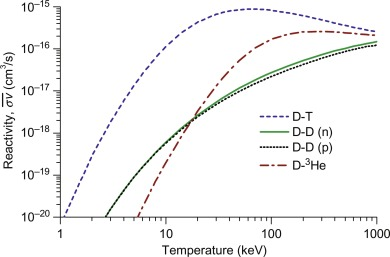
\includegraphics[width=12cm, height=9cm]{Reactividad.jpg}
        \end{figure}
        
        %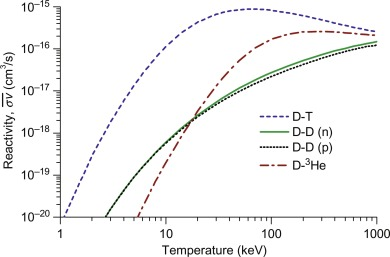
\includegraphics[width=7.5cm, height=5cm]{Reactividad.jpg} 

    Podemos observar, que de los procesos de reacción mostrados, la más conveniente de llevar a cabo es la de Deuterio-Tritio (D-T)pues tiene una mayor tasa de reacciones a ciertas temperaturas y además, para iniciarlas se requiere de menores cantidades de energía (Temperatura).
	%------------------------------------------
	\end{comment}

\end{document}